\documentclass[10pt,letterpaper,addpoints]{exam}
\usepackage[utf8]{inputenc}
\usepackage[spanish,es-noshorthands]{babel}
\usepackage{hyperref}
\usepackage{amsmath}
\usepackage{amsfonts}
\usepackage{amssymb}
\usepackage{graphicx}
\usepackage{tikz}
\usepackage{multicol}
\usepackage[width=7in,height=9.5in]{geometry}
%\printanswers
\begin{document}
\title{\begin{minipage}{.2\textwidth}
        
\includegraphics[height=1.75cm]{Images/logo-colegio.png}
       \end{minipage}
\begin{minipage}{.55\textwidth}
 \begin{center}
Prueba Bimestral ii\\Matem\'{a}ticas $11^{\circ}$
\end{center}
\end{minipage}
\begin{minipage}{.2\textwidth}

\includegraphics[height=1.75cm]{Images/logo-sed.png} 
\end{minipage}
}
\author{Germ\'{a}n Avendaño Ram\'{i}rez\\Lic. Matemáticas U.D., M.Sc. U.N.}
\date{}
\maketitle
\begin{center}
\fbox{\fbox{\parbox{5.5in}{\centering
Responda las preguntas en el cuadro de respuestas rellenando el \'{o}valo completamente. Debe hacer sus procedimientos en una hoja aparte.}}}
\end{center}
\vspace{0.1in}
\makebox[\textwidth]{Nombres: \hrulefill, curso:\underline{\hspace{48pt}}, fecha:\underline{\hspace{3cm}}}
Responda las preguntas \ref{preg-1} a \ref{preg-3} de acuerdo con la siguiente información
\begin{questions}
\begin{minipage}{.4\textwidth}
\question \label{preg-1}
El siguiente gráfico representa la posición respecto al tiempo de un cuerpo durante 12 segundos. El movimiento en tres intervalos de 4 segundos cada uno.\\

Respecto al movimiento realizado por el cuerpo en el intervalo de 4 a 8 segundos, podemos afirmar que
\end{minipage}\hfill
\begin{minipage}{.6\textwidth}
\begin{tikzpicture}[scale=0.75,yscale=0.5,xscale=0.8]
\draw[->] (0,0)node[left] {0} --(12.2,0) node[right]{$ t(s) $ };
\draw[<->] (0,-6.5) -- (0,8.5)node[left]{$ d(m) $};
\node[left]at(0,-6){-6};
\node[left]at(0,8){8};
\node[below] at (4,0){4};
\node[below] at (8,0){8};
\node[below] at (12,0){12};
\draw plot [domain=0:4] (\x, 2*\x);
\draw plot [domain=4:8] (\x,8);
\draw plot [domain=8:12](\x,-7/2*\x+36);
\draw[dashed](4,0)--(4,8);
\draw[dashed](8,0)--(8,8);
\draw[dashed](12,-6)--(12,0);
\draw[dashed](0,8)--(4,8);
\draw[dashed](0,-6)--(12,-6);
\end{tikzpicture}
\end{minipage}

\begin{choices}
\choice el cuerpo parte de la posición 4 y recorre con velocidad constante 8 metros.
\CorrectChoice el cuerpo permanece en reposo, ya que mantiene la misma posición, mientras transcurren los 4 segundos.
\choice el cuerpo cambia la dirección del movimiento y recorre 4 metros más en una superficie plana.
\choice el cuerpo recorre 4 metros con velocidad constante en 8 segundos.
\end{choices}
\question
Según la gráfica, se puede inferir que la velocidad del cuerpo en el transcurso de 8 a 12 segundos fue negativa, lo cual indica que
\begin{choices}
\choice el cuerpo disminuyó la velocidad que venía manteniendo en el intervalo de 4 a 8 segundos.
\CorrectChoice el cuerpo se devolvió seis metros más, desde el punto de partida.
\choice el cuerpo redujo el espacio recorrido durante los cuatro segundos respecto a los intervalos anteriores.
\choice el cuerpo recorrió la misma distancia, pero empleó más tiempo que en los intervalos anteriores.
\end{choices}
\question \label{preg-3}
En el intervalo de 12 a 16 segundos se produjo un movimiento representado por la función: $ f(t)=\frac{3}{4}t-15 $. La interpretación de este movimiento realizado por el cuerpo es
\begin{choices}
\CorrectChoice el cuerpo recorrió tres metros durante los cuatro segundos
\choice el cuerpo incrementó su velocidad en 5 metros por cada segundo
\choice el cuerpo retrocedió 15 metros durante el intervalo de tiempo.
\choice el cuerpo disminuyó su velocidad en dos metros durante los cuatro segundos.
\end{choices}
\question
Sean\\
  \textbf{P} la gráfica de la función $ y=x^2-2x+3 $\\
  \textbf{Q} la gráfica de la función $ y=x^2+2x+1 $\\
  Considere las siguientes afirmaciones suponiendo que \textbf{P} y \textbf{Q} están trazadas en el mismo sistema de coordenadas
  \begin{itemize}\begin{multicols}{2}
    \item[I] \textbf{P} y \textbf{Q} coinciden
    \item[II] \textbf{P} está a la izquierda de \textbf{Q}
    \item[III] \textbf{P} está a la derecha de \textbf{Q}
    \item[IV] \textbf{P} está más arriba que \textbf{Q}
    \item[V] \textbf{P} está más abajo que \textbf{Q}
  \end{multicols}
  \end{itemize}
  De las anteriores afirmaciones es o son verdaderas

  \begin{oneparchoices}
\choice sólo I
\choice II y V
\choice II y IV
\CorrectChoice III y IV  
  \end{oneparchoices}
  \question Una compañía de taxis cobra una tarifa de \$3.000 por el primer kilómetro o fracción de kilómetro recorrida y \$1.000 por cada kilómetro o fracción adicional. ¿Cuál de las siguientes gráficas representa la relación entre el costo de un viaje $y$ y el número de kilómetros recorridos $x$?
  
  \begin{minipage}{0.45\textwidth}
  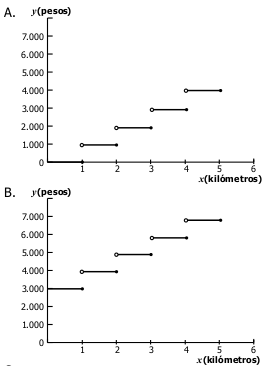
\includegraphics[scale=.65]{Images/grafica-taxi.png}
\end{minipage}\hfill
\begin{minipage}{.45\textwidth}
  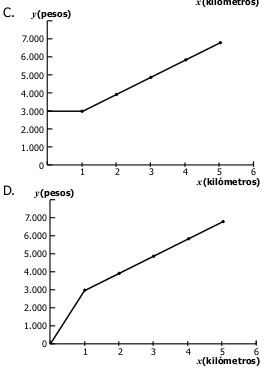
\includegraphics[scale=.65]{Images/grafica-taxi-2.png}
\end{minipage}
%\begin{oneparchoices}
%\choice[1] Nunca
%\end{oneparchoices}
%\answerline
\end{questions}
%cuadro de puntajes
%\begin{center}
%\gradetable[h][pages]
%\end{center}
\end{document}